\section{設計}
システムは図~\ref{fig:system_fig}のように設定し,
Raspberry PiをWifiを通してネットワーク
接続,サーバーとして稼働させることでネットワークに
接続している外部の機器と通信する.
遠隔操作のインターフェースとしてWebアプリケーションを作成し,
鍵の共有はWebアプリケーションにおけるアクセス権の共有という
形で実現した.

% system figure
\begin{figure}[htbp]
  \centering
  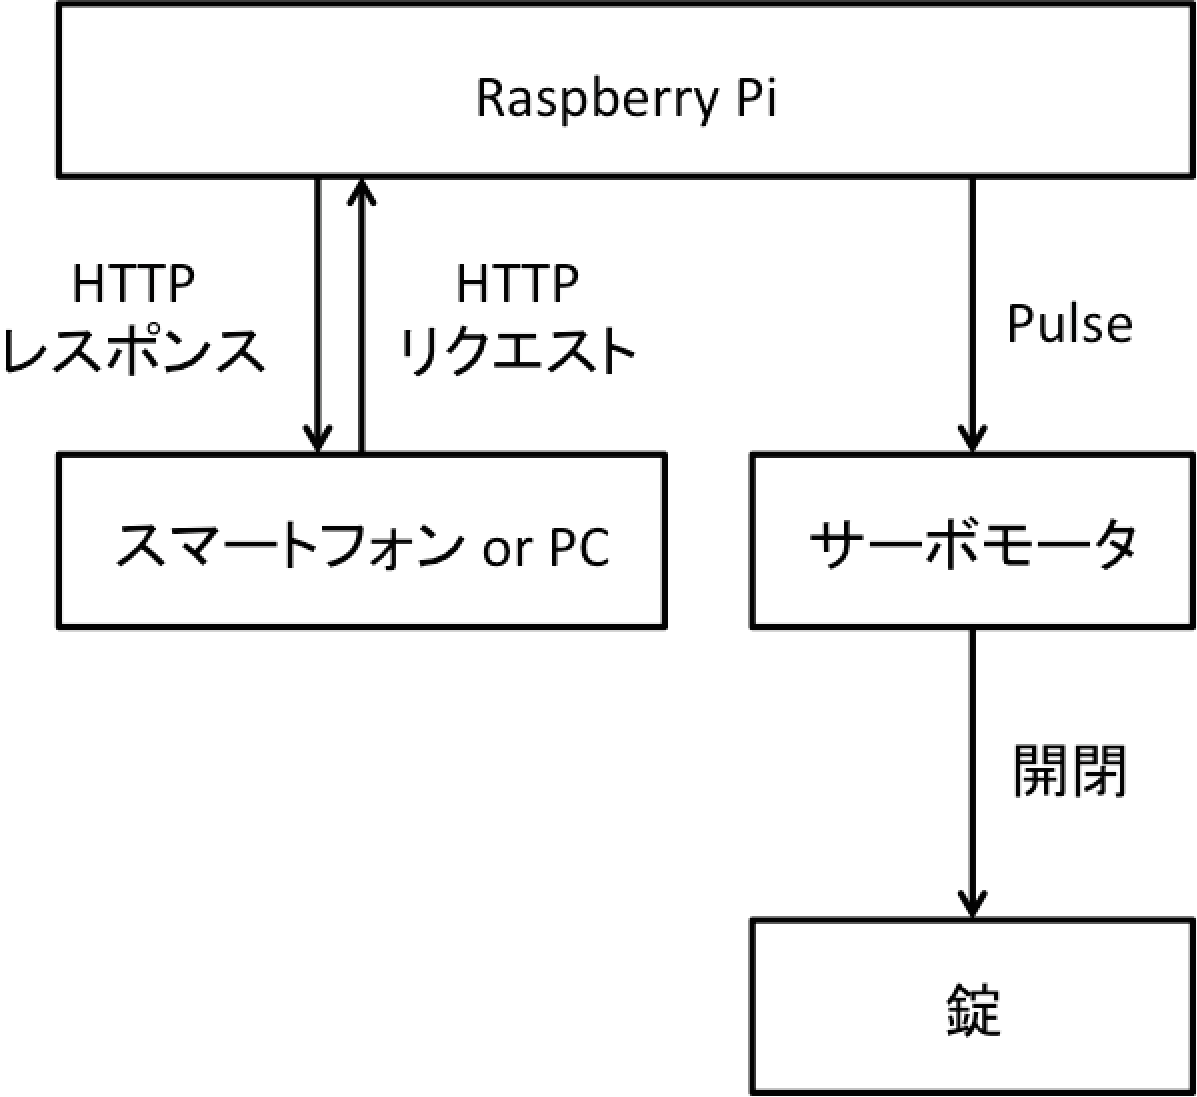
\includegraphics[width=0.35\textwidth]{./assets/system_fig.eps}
  \caption{システム図}
  \label{fig:system_fig}
\end{figure}

\subsection{モーター}
モーターはピンの消費が少なく外部電源の必要ないサーボモータを利用した.
サーボモータは図~\ref{fig:servo}, 表~\ref{tbl:servo_specifications}
のような仕様のものを利用し,
解錠に必要なトルクとスピードを満たすものを選択した.

\begin{figure}[htbp]
  \centering
  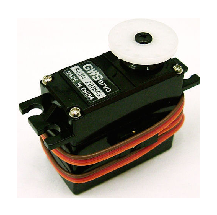
\includegraphics[width=0.2\textwidth]{./assets/servo.eps}
  \caption{サーボモータ}
  \label{fig:servo}
\end{figure}

\begin{table}[htbp]
  \begin{center}
    \begin{tabular}{cc}
      Torque & 3.4 kg (4.8V)  \\
      Weight & 64 g  \\
      Speed  & 0.23 sec / 60 deg (4.8V) \\
      Size   & 39.5 x 20 x 35.6 mm
    \end{tabular}
    \caption{GWSサーボ S03N/2BBMG/JRタイプ}
    \label{tbl:servo_specifications}
  \end{center}
\end{table}

\subsection{Webアプリケーション}
外部機器との通信において,モータの操作や鍵の共有
を行うためのインターフェースとしてWebアプリケーションを作成した.
作成したWebページは以下4ページである.

\begin{itemize}[noitemsep]
  \item ログインページ.(図~\ref{fig:login_page})
  \item 錠の状態,開閉操作ページ.(図~\ref{fig:control_page})
  \item ログ確認ページ.(図~\ref{fig:log_page})
  \item アクセス権付与ページ.(図~\ref{fig:authorize_page})
\end{itemize}

ログインは独自のアカウントは作成せず,Googleアカウントで行う.
Google APIを使ってメールアドレスや名前,プロフィール画像などが取得可能
であるため,基本情報などの入力なしにスムーズに利用へ
移ることができる.
共有はアクセス権のある者がメールアドレスを入力して与えるという形をとる.

また,錠の状態と開閉の操作ページ(図~\ref{fig:control_page})において,
多人数が利用することを考慮し,ブラウザの更新なしに開閉状態が
切り替わるようにした.
これはAjaxを用いて定期的にデータベース内の情報を取得することで実現した.

\begin{figure}[htbp]
  \begin{tabular}{cc}
    \begin{minipage}{0.5\hsize}
      \begin{center}
        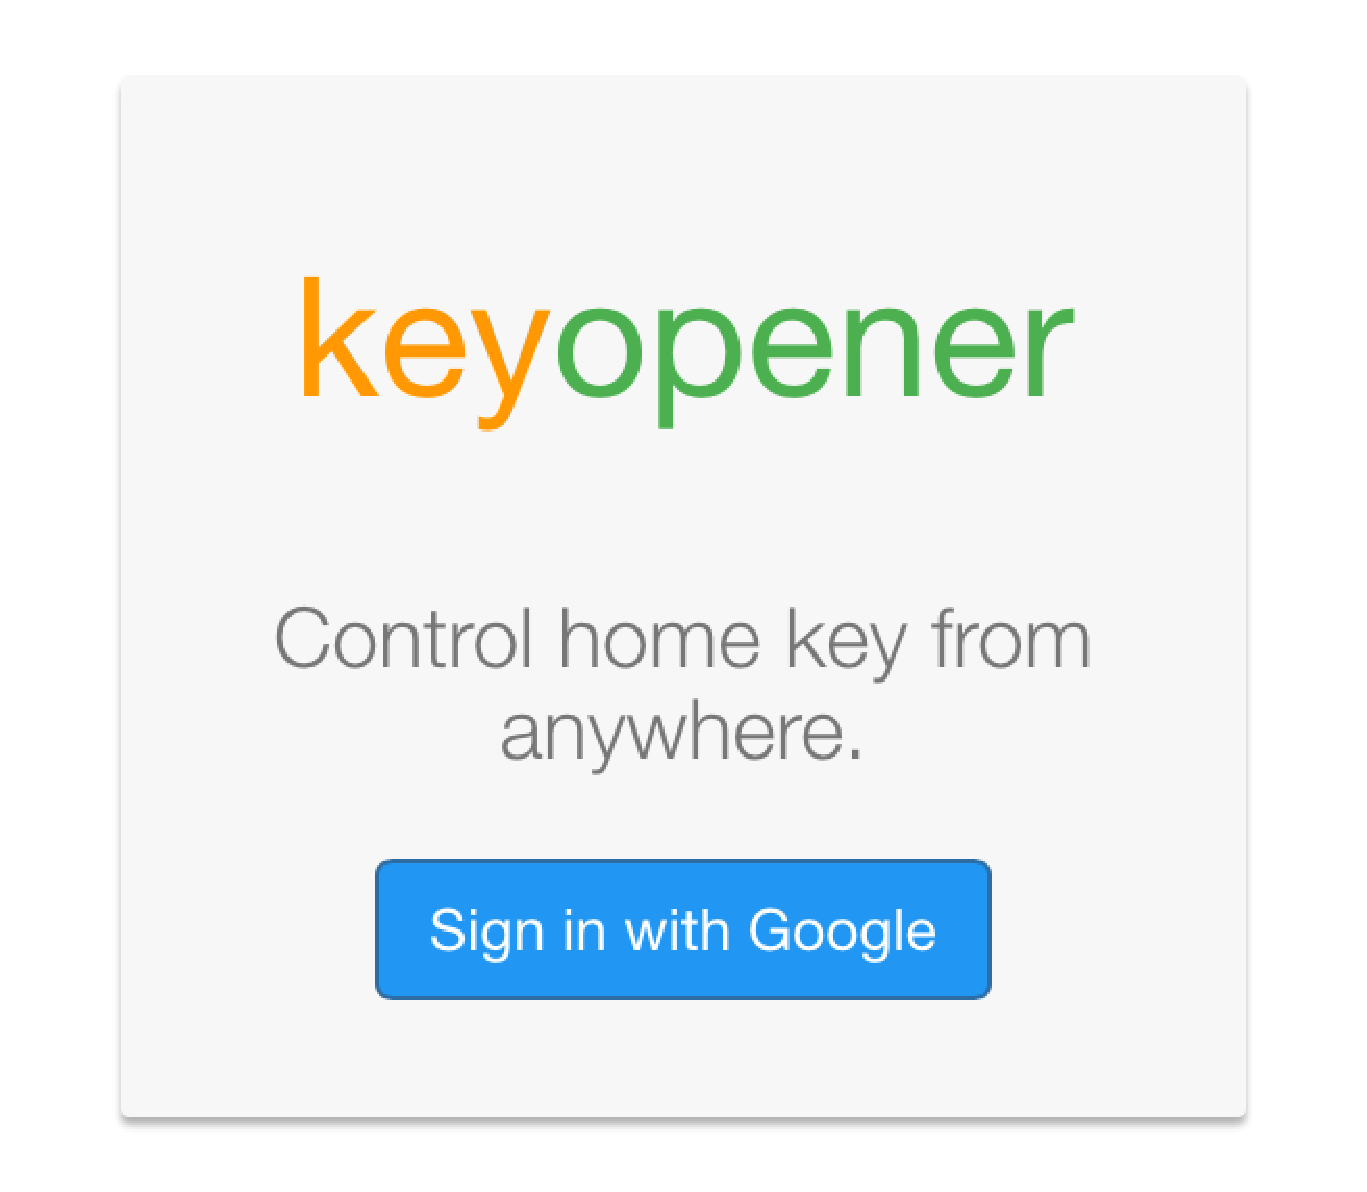
\includegraphics[width=0.8\textwidth]{./assets/login_page.eps}
        \caption{ログイン}
        \label{fig:login_page}
      \end{center}
    \end{minipage}
    \begin{minipage}{0.5\hsize}
      \begin{center}
        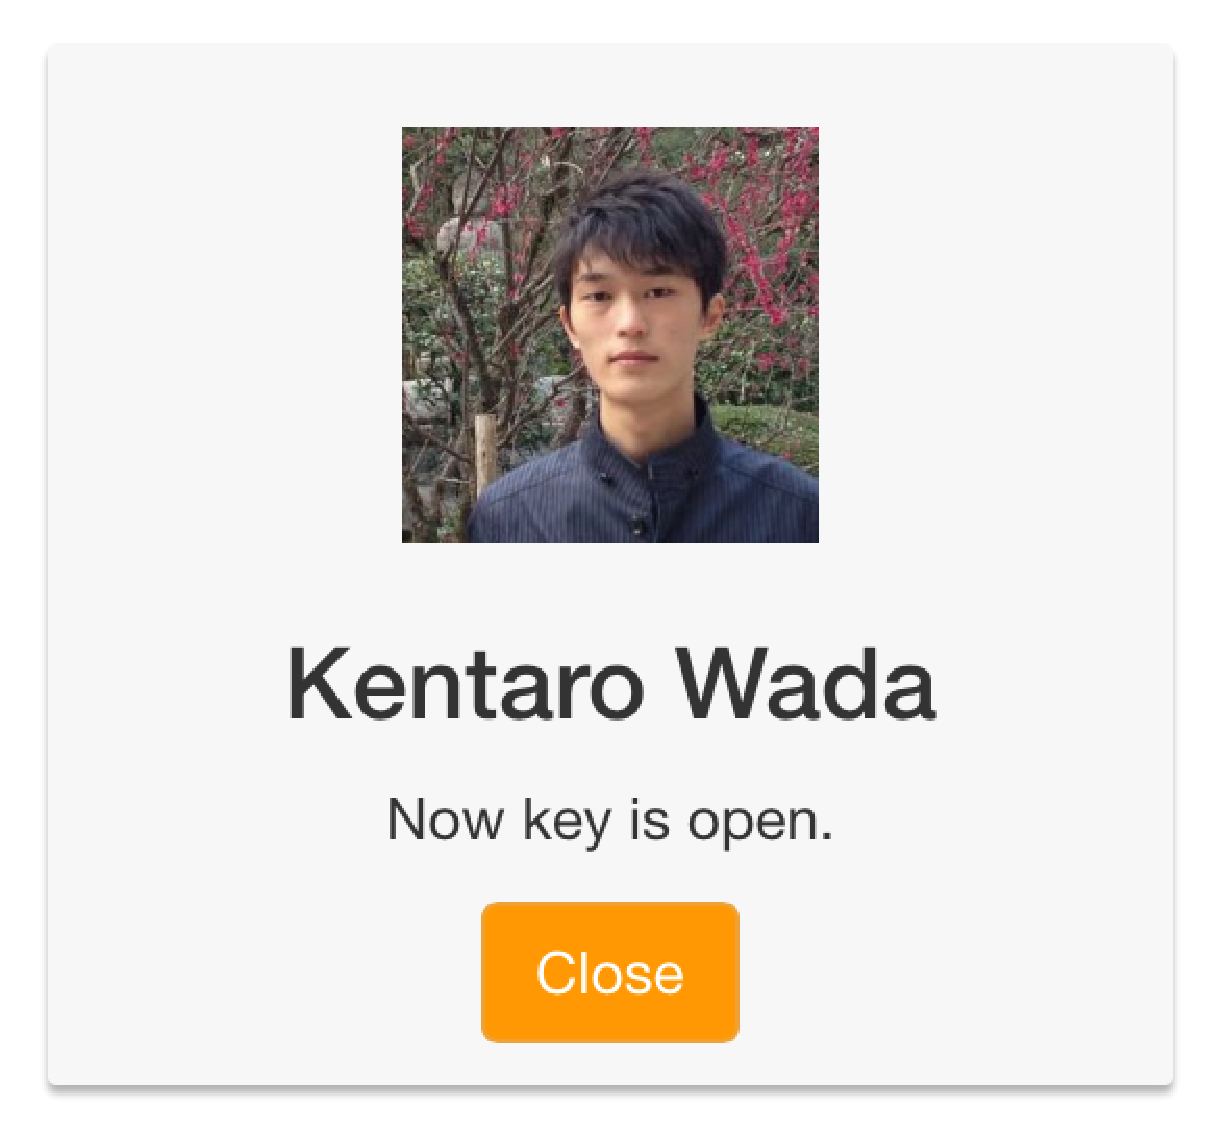
\includegraphics[width=0.75\textwidth]{./assets/control_page.eps}
        \caption{状態,開閉操作}
        \label{fig:control_page}
      \end{center}
    \end{minipage}
  \end{tabular}
\end{figure}

\begin{figure}[htbp]
  \begin{tabular}{cc}
    \begin{minipage}{0.5\hsize}
      \begin{center}
        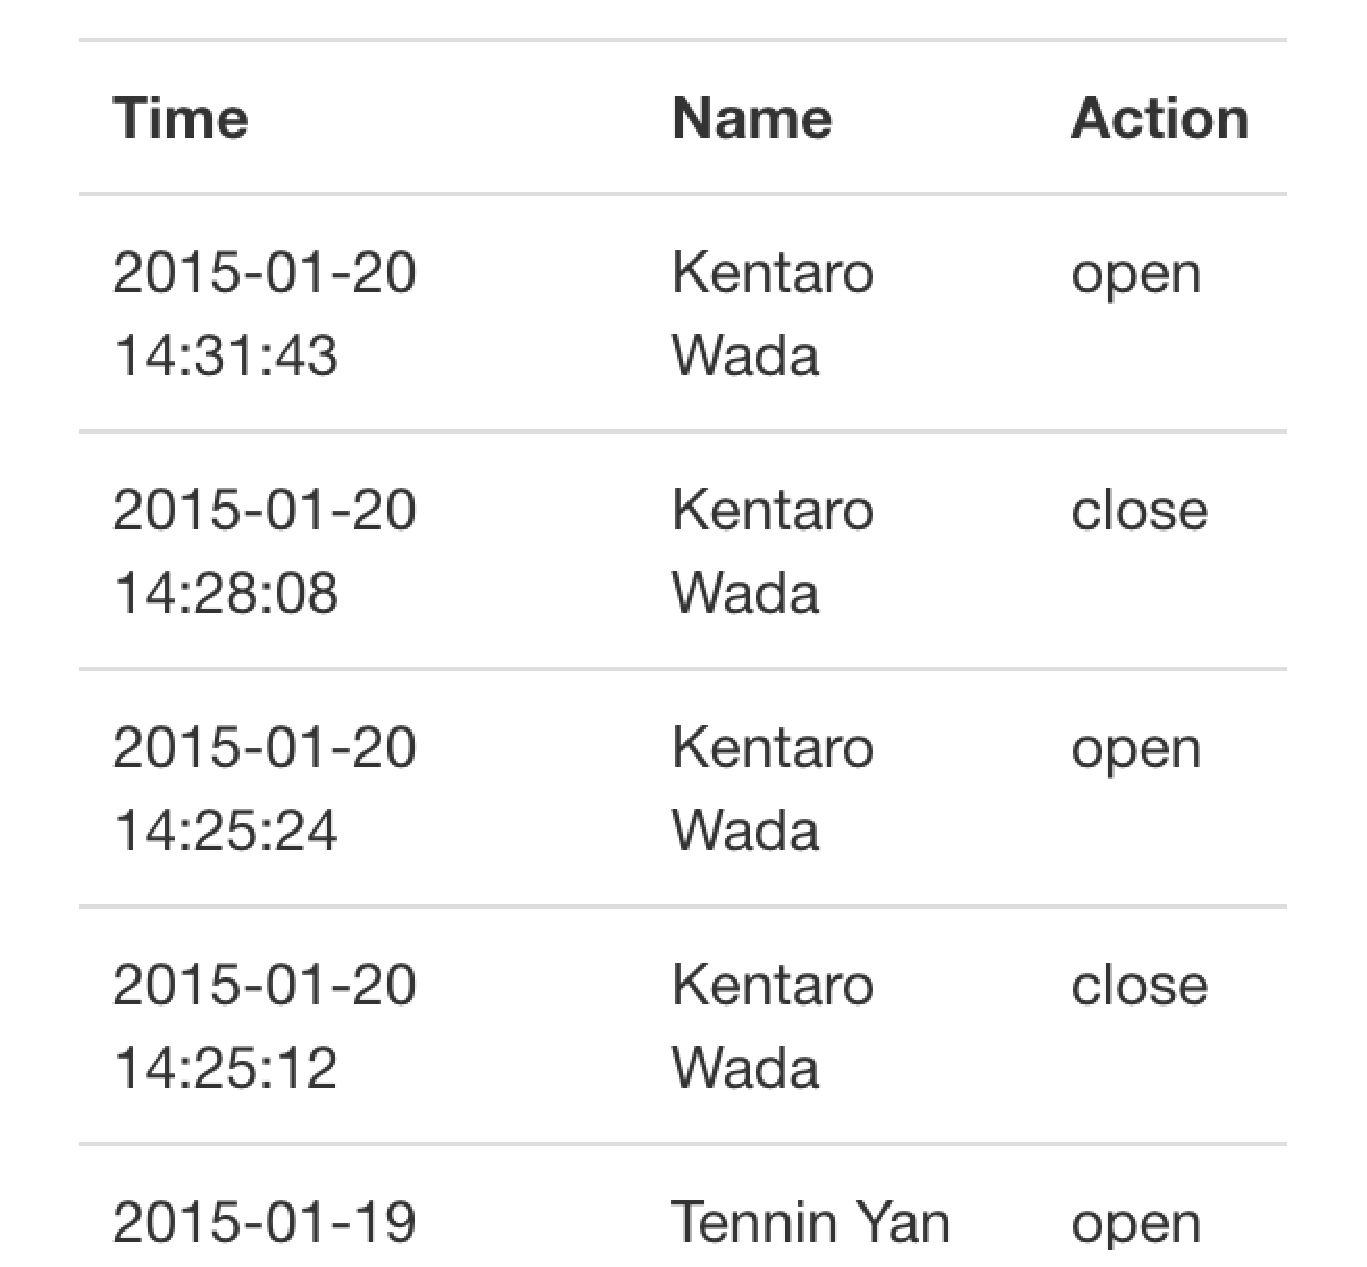
\includegraphics[width=0.7\textwidth]{./assets/log_page.eps}
        \caption{ログ確認}
        \label{fig:log_page}
      \end{center}
    \end{minipage}
    \begin{minipage}{0.5\hsize}
      \begin{center}
        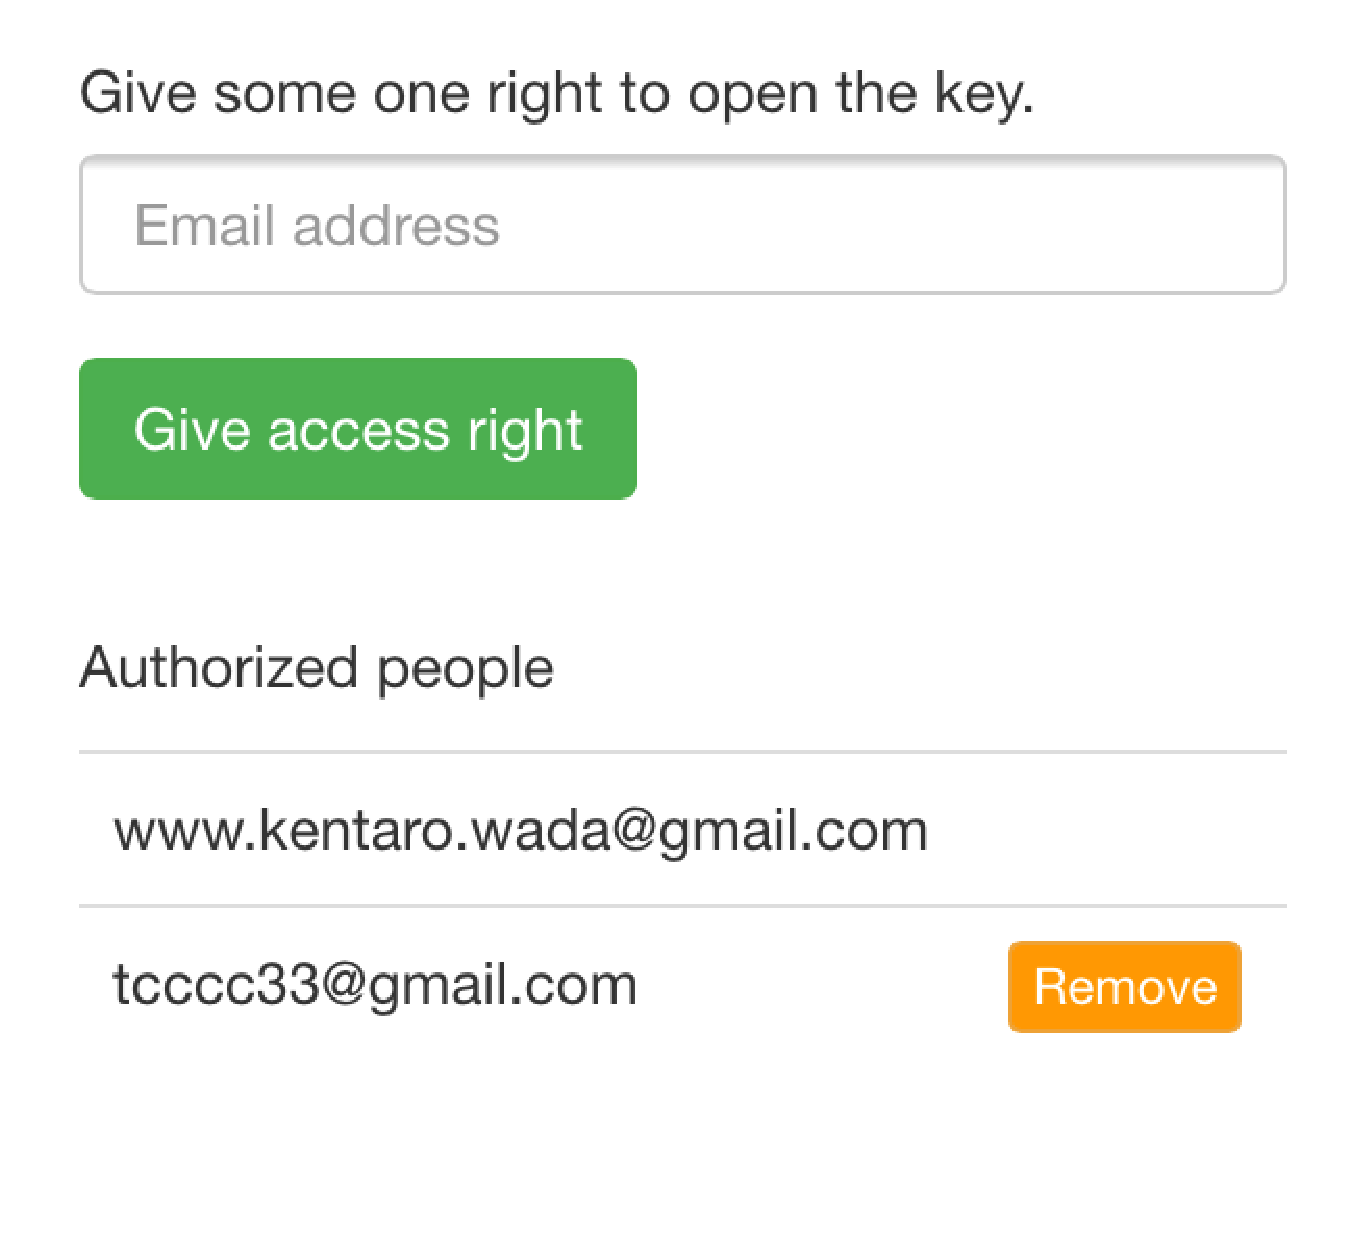
\includegraphics[width=0.7\textwidth]{./assets/authorize_page.eps}
        \caption{アクセス権付与}
        \label{fig:authorize_page}
      \end{center}
    \end{minipage}
  \end{tabular}
\end{figure}

\subsection{取付機構}
取付機構に関して,以下の点に留意した.

\begin{itemize}[noitemsep]
  \item 取り付けが容易であること.
  \item 不可逆な変形を伴わないこと.
  \item 多くのドアに対応できること.
\end{itemize}

機構は大きく図~\ref{fig:head},~\ref{fig:foot}
の二つからなっており,それぞれサムーンとドアノブに取り付ける.
サムターンとはドアの内側に付いている,錠の開閉に使う金具のことである.

サムターンへの取付部は,デバイスの自重を支えるためのものであり,
ネジで締めることでサムターンに固定される.
ドアノブ取付部は,モーター本体の回転を固定するためのもので,これによって
モーターの本体部は回転せず,サムターンに固定されている部分が回転し,
鍵が開くという仕組みである.

\begin{figure}[htbp]
  \begin{tabular}{cc}
    \begin{minipage}{0.5\hsize}
      \begin{center}
        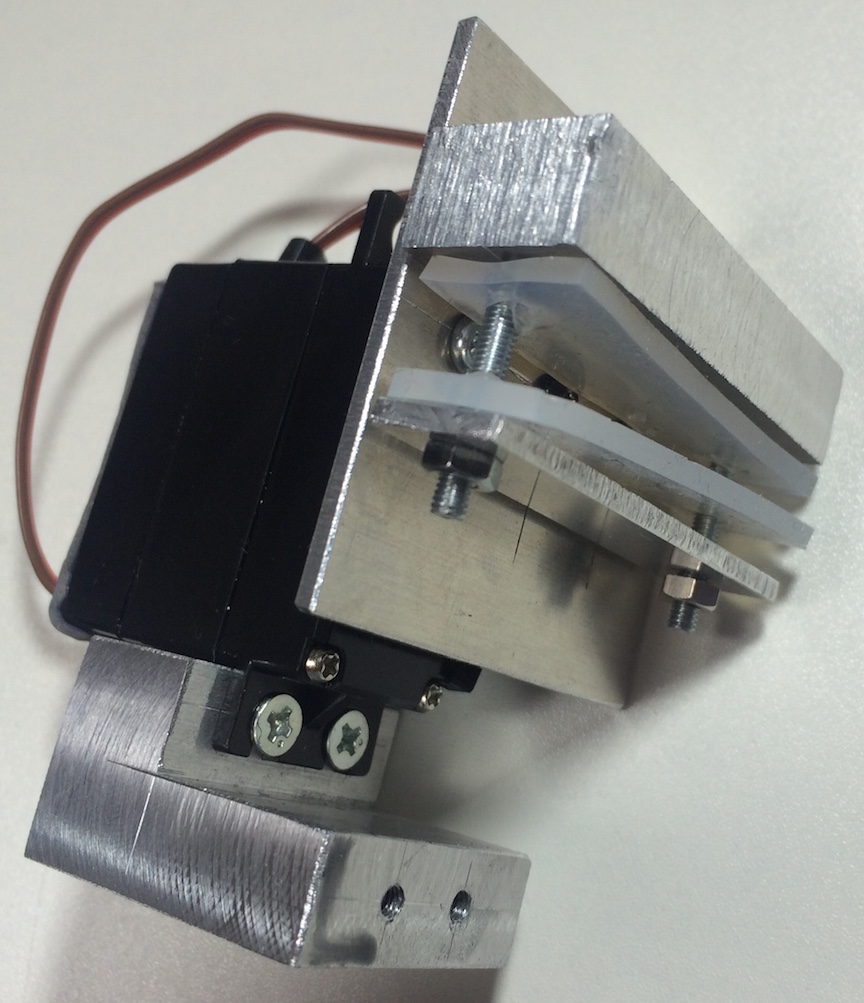
\includegraphics[width=0.6\textwidth]{./assets/head.eps}
        \caption{サムターン取付部}
        \label{fig:head}
      \end{center}
    \end{minipage}
    \begin{minipage}{0.5\hsize}
      \begin{center}
        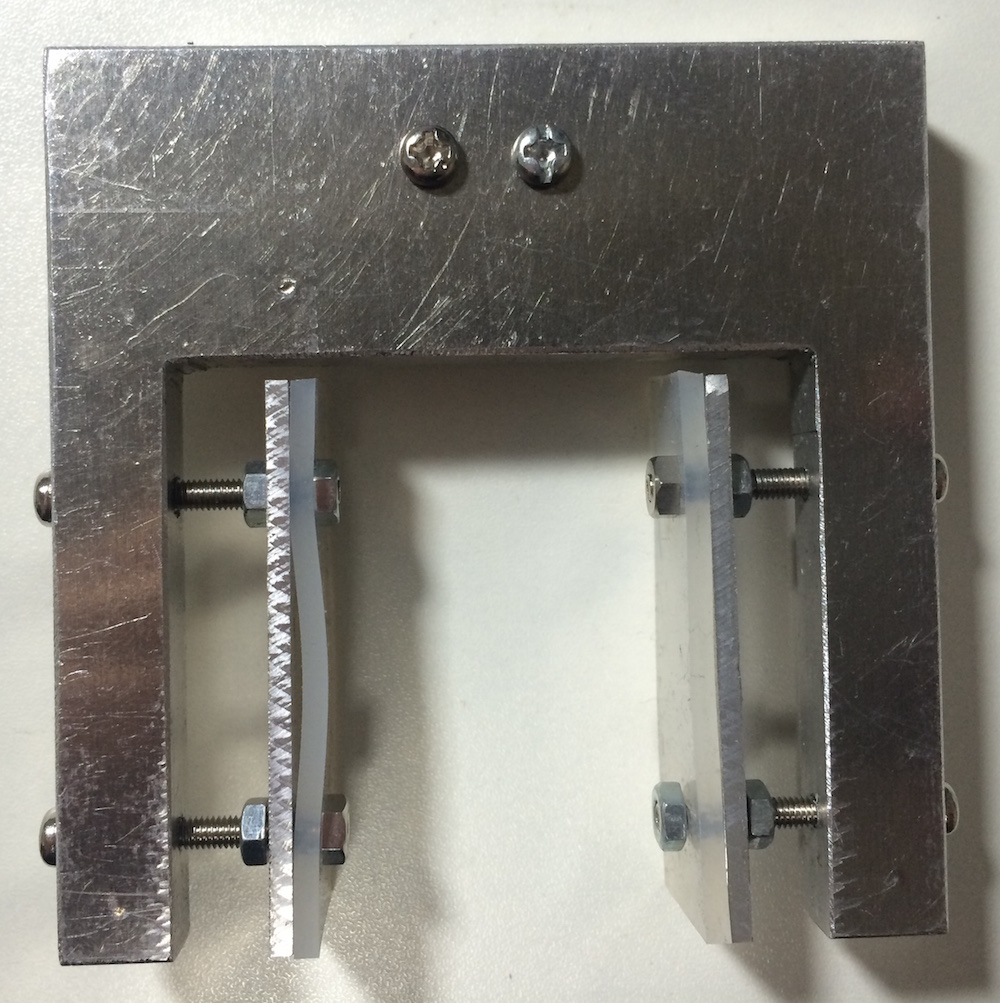
\includegraphics[width=0.7\textwidth]{./assets/foot.eps}
        \caption{ドアノブ取付部}
        \label{fig:foot}
      \end{center}
    \end{minipage}
  \end{tabular}
\end{figure}

\subsection{バッテリー}
バッテリーは図~\ref{fig:battery}, 表~\ref{tbl:battery}に示す,
モバイルバッテリーを採用した.

\begin{figure}[htbp]
  \centering
  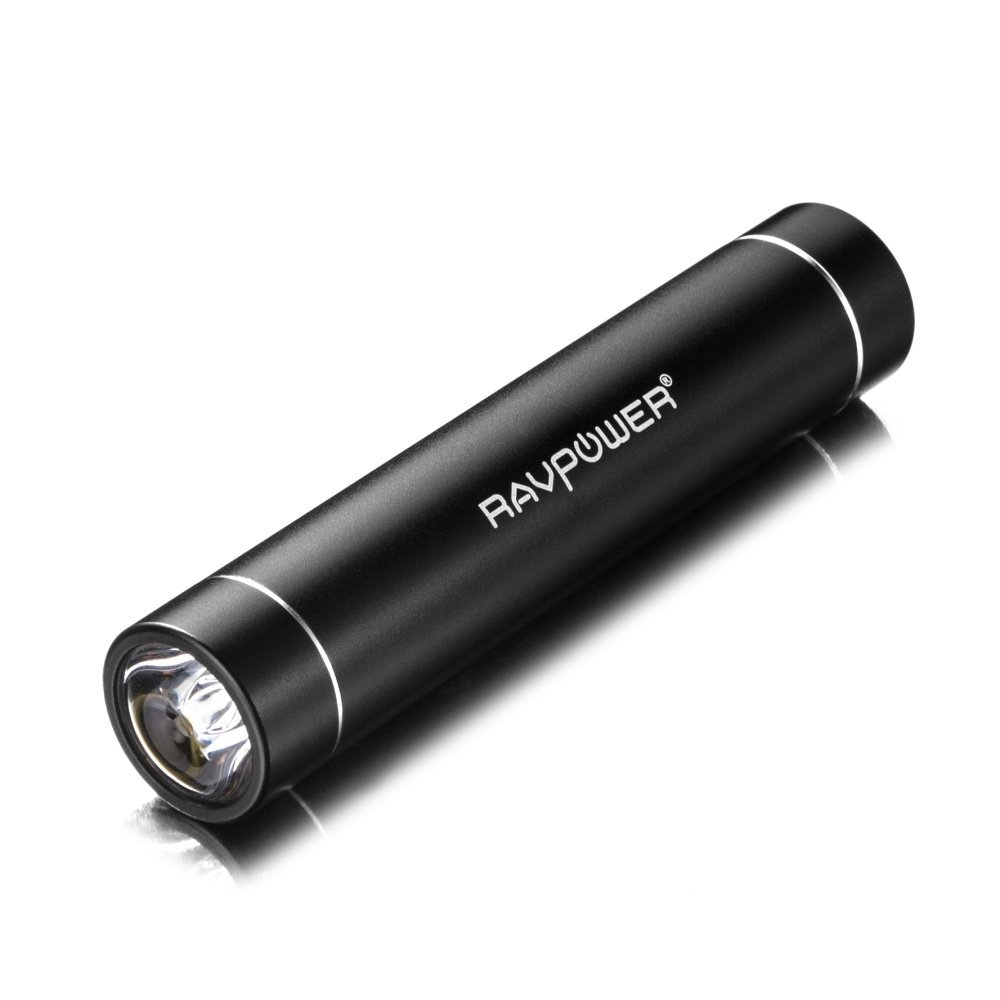
\includegraphics[width=0.2\textwidth]{./assets/battery.eps}
  \caption{バッテリー}
  \label{fig:battery}
\end{figure}

\begin{table}[htbp]
  \begin{center}
    \begin{tabular}{cc}
      Capacity & 3200 mAh \\
      Weight & 73 g \\
      Size & 108 x 22 x 22 mm \\
    \end{tabular}
    \caption{バッテリー仕様}
    \label{tbl:battery}
  \end{center}
\end{table}

